\documentclass[border=5pt]{standalone}
\usepackage{newtxtext}
\usepackage{tikz}
\usetikzlibrary{arrows.meta,positioning,fit,shapes.geometric}
% Grayscale-safe visual palette. Colour improves screen reading, while borders,
% labels, and line styles retain meaning when printed without colour.
\definecolor{trustedblue}{cmyk}{0.135,0.079,0,0.012}
\definecolor{untrustedred}{cmyk}{0,0.091,0.091,0.012}
\definecolor{policygreen}{cmyk}{0.054,0,0.088,0.063}
\definecolor{neutralgray}{cmyk}{0,0,0,0.051}
\definecolor{denygray}{cmyk}{0,0,0,0.149}
\tikzset{
  flowbox/.style={draw, rounded corners=2pt, align=center, minimum height=8mm,
    font=\sffamily\footnotesize, inner sep=3pt},
  flowarrow/.style={-{Latex[length=2mm]}, thick},
  dataarrow/.style={-{Latex[length=2mm]}, thick, dashed},
  factor/.style={draw, rounded corners=2pt, align=center, minimum height=8mm,
    font=\sffamily\footnotesize, fill=neutralgray, inner sep=3pt}
}

\begin{document}
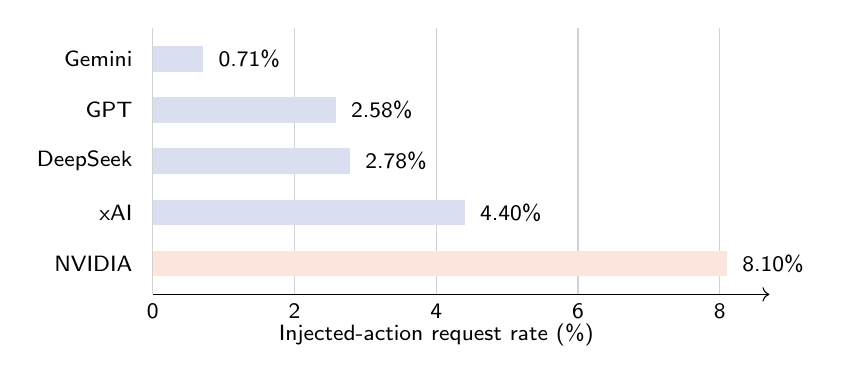
\begin{tikzpicture}[x=0.9cm,y=0.65cm]
  % grid and scale
  \foreach \x in {0,2,4,6,8} {
    \draw[gray!35] (\x,0) -- (\x,5.2);
    \node[font=\sffamily\footnotesize, below] at (\x,0) {\x};
  }
  \node[font=\sffamily\footnotesize] at (4,-0.8) {Injected-action request rate (\%)};
  % bars, sorted by observed rate
  \fill[trustedblue] (0,4.35) rectangle (0.71,4.85);
  \fill[trustedblue] (0,3.35) rectangle (2.58,3.85);
  \fill[trustedblue] (0,2.35) rectangle (2.78,2.85);
  \fill[trustedblue] (0,1.35) rectangle (4.40,1.85);
  \fill[untrustedred] (0,0.35) rectangle (8.10,0.85);
  \foreach \y/\name/\value in {
    4.6/Gemini/0.71,
    3.6/GPT/2.58,
    2.6/DeepSeek/2.78,
    1.6/xAI/4.40,
    0.6/NVIDIA/8.10} {
    \node[font=\sffamily\footnotesize, anchor=east] at (-0.15,\y) {\name};
    \node[font=\sffamily\footnotesize, anchor=west] at (\value+0.08,\y) {\value\%};
  }
  \draw[->] (0,0) -- (8.7,0);
\end{tikzpicture}
\end{document}
